\documentclass[border=4pt]{standalone}
\usepackage[utf8]{inputenc}\usepackage[T1]{fontenc}\usepackage{mathptmx}
\usepackage{tikz}\usetikzlibrary{positioning,arrows.meta,calc,fit}
\begin{document}
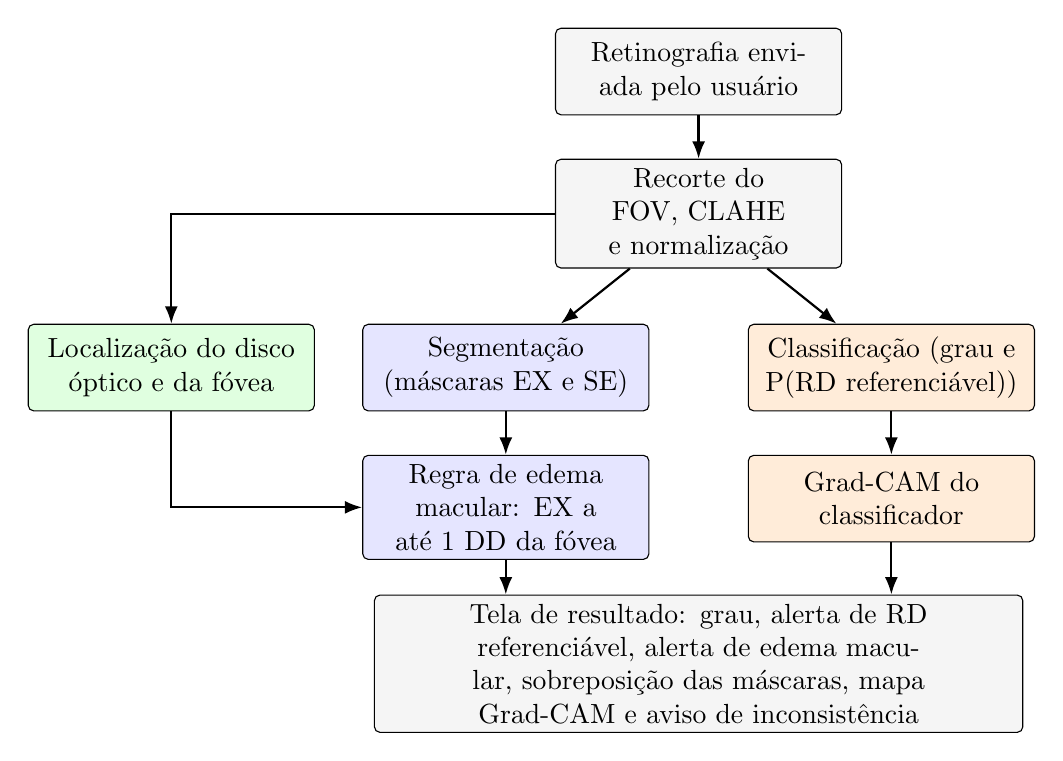
\begin{tikzpicture}[font=\normalsize,node distance=0.55cm and 0.6cm,
  b/.style={draw,rounded corners=2pt,align=center,text width=3.4cm,minimum height=1.1cm,fill=#1},b/.default=gray!8,
  arr/.style={-{Latex[length=2.2mm]},thick}]
\node[b] (in) {Retinografia enviada pelo usuário};
\node[b,below=of in] (pre) {Recorte do FOV, CLAHE e normalização};
\node[b=blue!10,below left=0.7cm and -1.2cm of pre] (seg) {Segmentação (máscaras EX e SE)};
\node[b=orange!15,below right=0.7cm and -1.2cm of pre] (clf) {Classificação (grau e P(RD referenciável))};
\node[b=green!12,left=of seg] (loc) {Localização do disco óptico e da fóvea};
\node[b=blue!10,below=of seg] (dme) {Regra de edema macular: EX a até 1 DD da fóvea};
\node[b=orange!15,below=of clf] (cam) {Grad-CAM do classificador};
\node[b,below=of $(dme.south)!0.5!(cam.south)$,text width=8.0cm] (out) {Tela de resultado: grau, alerta de RD referenciável, alerta de edema macular, sobreposição das máscaras, mapa Grad-CAM e aviso de inconsistência};
\draw[arr] (in)--(pre); \draw[arr] (pre)--(seg); \draw[arr] (pre)--(clf); \draw[arr] (pre.west) -| (loc.north);
\draw[arr] (seg)--(dme); \draw[arr] (loc)|-(dme); \draw[arr] (clf)--(cam);
\draw[arr] (dme.south)--(dme.south|-out.north); \draw[arr] (cam.south)--(cam.south|-out.north);
\end{tikzpicture}
\end{document}
